\chapter{Testprotokoll Sprint 1}
\section{Test}
\subsection{Angaben zum Test}

\begin{tabularx}{\linewidth}{l l l}
\textbf{datum des Builds} & \textbf{Tester} & \textbf{datum der Testdurchführung}\\
\hline
02.11.15 & Silvan Adrian & 02.11.15

\end{tabularx}

\subsection{Zusammenfassung Ergebnis}
\begin{tabularx}{\linewidth}{l l l}
\textbf{Test durchgeführt?} & \textbf{Tests erfolgreich?} & \textbf{Tests fehlgeschalgen?}\\
\hline
5 (alle) & 5 (alle) & 0 \\
\hline
\end{tabularx}


\subsection{Ergebnisse Tests}
\begin{tabularx}{\linewidth}{l l l}
\textbf{Was} & \textbf{Ok? / nicht OK?} & \textbf{Aufgetretene Fehler}\\
\hline
\textbf{Unit-Tests} & {\color{green} OK}  & keine\\
\hline
Systemtest 1: & & \\
\textbf{Testservice abonnieren} & {\color{green} OK} & keine\\
\hline
Systemtest 2: & & \\
\textbf{Testservice kündigen} & {\color{green} OK}  & keine\\
\hline
Systemtest 3: & & \\
\textbf{Abonnierte Services anzeigen} & {\color{green} OK}  & keine\\
\hline
Systemtest 4: & & \\
\textbf{Verfügbare Services anzeigen} & {\color{green} OK}  & keine\\
\hline



\end{tabularx}

\newpage

\section{Metriken}
Die abschliessenden Metriken vom Sprint aus SonarQube.
\subsection{Projekt in Zahlen}
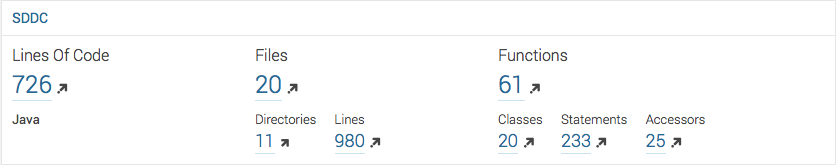
\includegraphics[]{loc}

\subsection{Unit Tests Coverage}
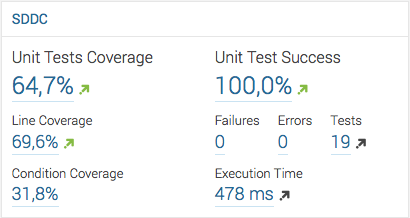
\includegraphics[]{./10_Protokolle/04_Testprotokoll/images/Sprint1/coverage}

\subsection{Coverage Verteilung auf einzelne Dateien}
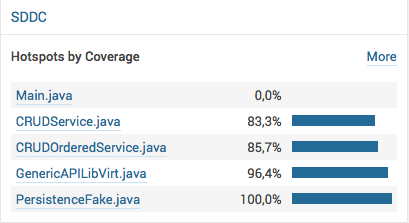
\includegraphics[]{./10_Protokolle/04_Testprotokoll/images/Sprint1/covergaeperfile}

\subsection{Findbugs Issues}
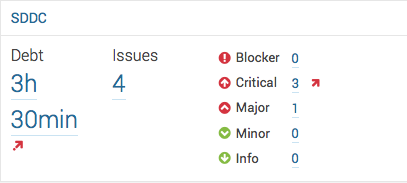
\includegraphics[]{./10_Protokolle/04_Testprotokoll/images/Sprint1/issues}
\subsubsection{Issues}
\textbf{HashCode}\\
Da es sich hierbei nur um einen Persistance Fake handelt wurde drauf verzichtet 
das Issue zu beheben und wird im nächsten Sprint sowieso entfernt.
\newline
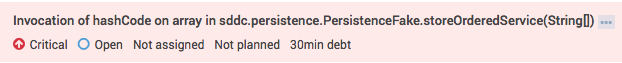
\includegraphics[width=\textwidth]{./10_Protokolle/04_Testprotokoll/images/Sprint1/hashcode}
\newline
\textbf{Encoding}\\
Issue besteht im Main File. welches im nächsten Sprint nicht mehr so existiert.
\newline
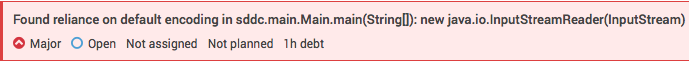
\includegraphics[width=\textwidth]{./10_Protokolle/04_Testprotokoll/images/Sprint1/encoding}
\newline
\textbf{Infiniteloop}\\
Für die Konsolen Eingaben wurde ein Infinite Loop erstellt, welcher es einem 
erlaubt mehrmals Eingaben zu machen.
\newline
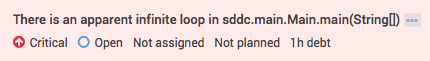
\includegraphics[width=\textwidth]{./10_Protokolle/04_Testprotokoll/images/Sprint1/infiniteloop}
\newline
\textbf{Null Check}\\
Ebenfalls im Main java File, welches noch abgeändert und nicht mehr in dieser 
Konstellation existieren wird.
\newline
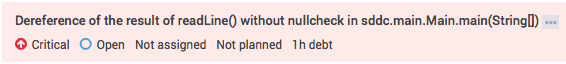
\includegraphics[width=\textwidth]{./10_Protokolle/04_Testprotokoll/images/Sprint1/nullcheck}

\section{Kommentare}

Die Konsolen App bietet ganz einfach Eingaben und Möglichkeiten die Service 
abonnieren und kündigen zu können.
Verbesserungen werden im Code Review Dokument beschrieben.
